\chapter{Handbuch: Benutzung des Programms} \label{chp:handbook}


\section{Konfigurationsoberfläche}
\subsection{Anzeigen und ändern eines Endpunktes}
Nach dem Aufrufen der Administrationsoberfläche, sind entweder vorhandene Tabellen gelistet oder es wird, bei nichtvorhandensein von Tabellen, nur die Kopfleiste angezeigt. 

In \autoref{fig:hb_1} ist bereits ein Endpunkt zu sehen: \textit{artikel}. 

\begin{figure}[h]
    \centering
    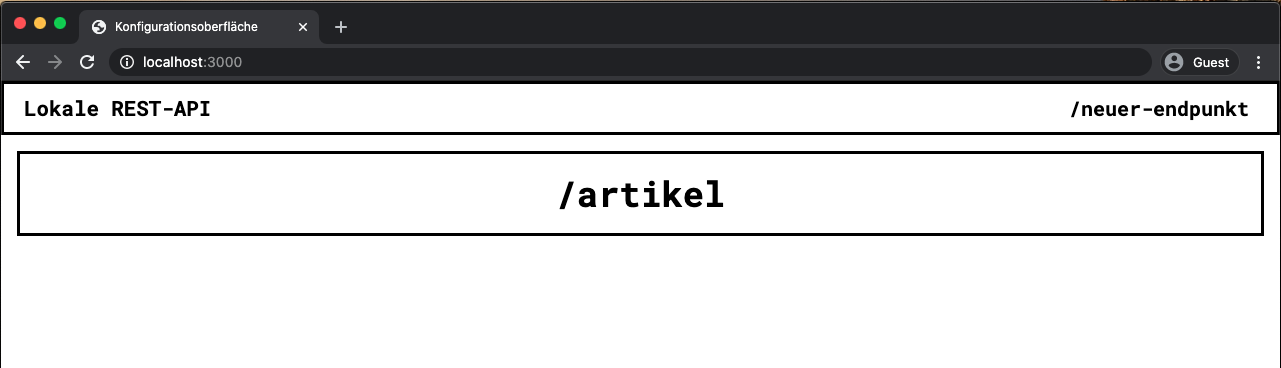
\includegraphics[width=15cm]{figures/hb_1.png}    %0.6\textwidth
    \caption{Startbildschirm der Administrationsoberfläche}
    \label{fig:hb_1}
\end{figure}

Mit einem Klick auf diesen Endpunkt wird eine Übersicht über die Benutzung angezeigt. Die verschiedene Spalten geben Auskunft über die zu verwendende Methode und dem Pfad. Zudem gibt es eine Spalte \textit{Beschreibung} in der noch einmal beschrieben wird wie die jeweilige Methode zu nutzen ist. Eine genaue Erklärung zur Nutzung der \gls{api} erfolgt im \autoref{chp:conclusion}.

\begin{figure}[H]
    \centering
    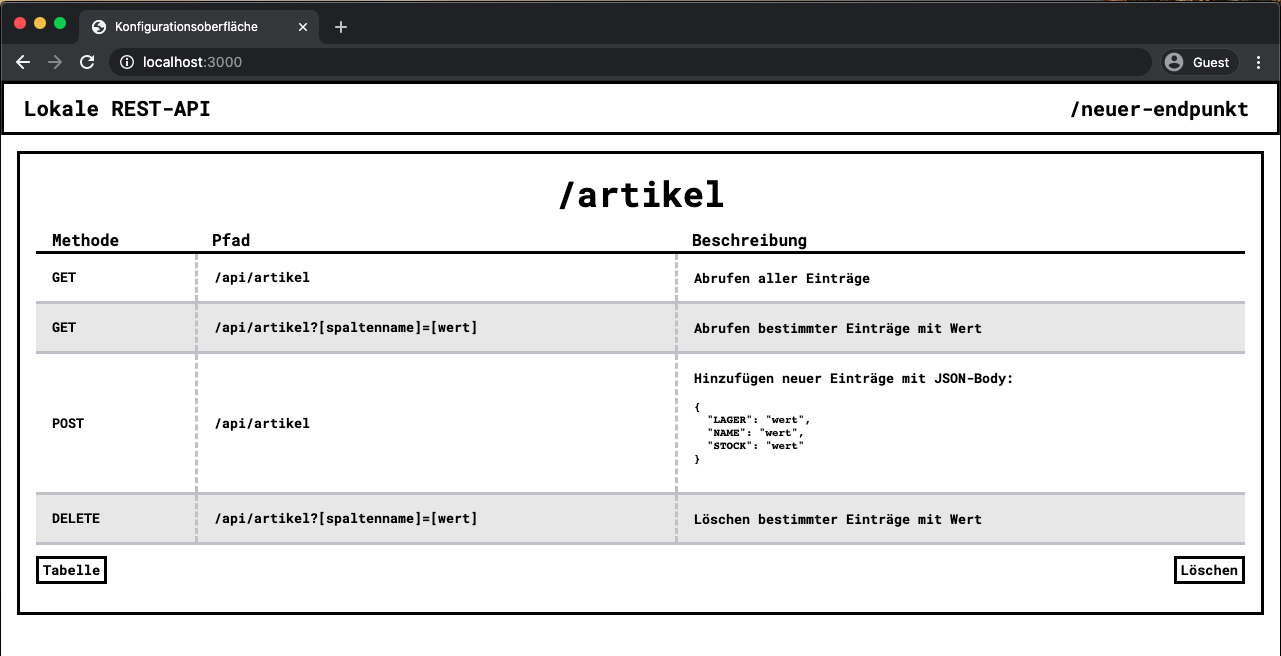
\includegraphics[width=15cm]{figures/hb_2.png}    %0.6\textwidth
    \caption{Anzeige eines Endpunktes}
    \label{fig:hb_2}
\end{figure}

Mit einem Klick auf den Button \textit{Tabelle}, öffnet sich ein Modal in dem die dazugehörigen Daten stehen (\autoref{fig:hb_3}). Oben links lässt sich die Form der Tabelle einsehen - in diesem Fall 4 Spalten und 4 Zeilen. Durch ändern der Zahlen können hier beliebig Zeilen hinzugefügt oder entfernt werden. 

\begin{figure}[H]
    \centering
    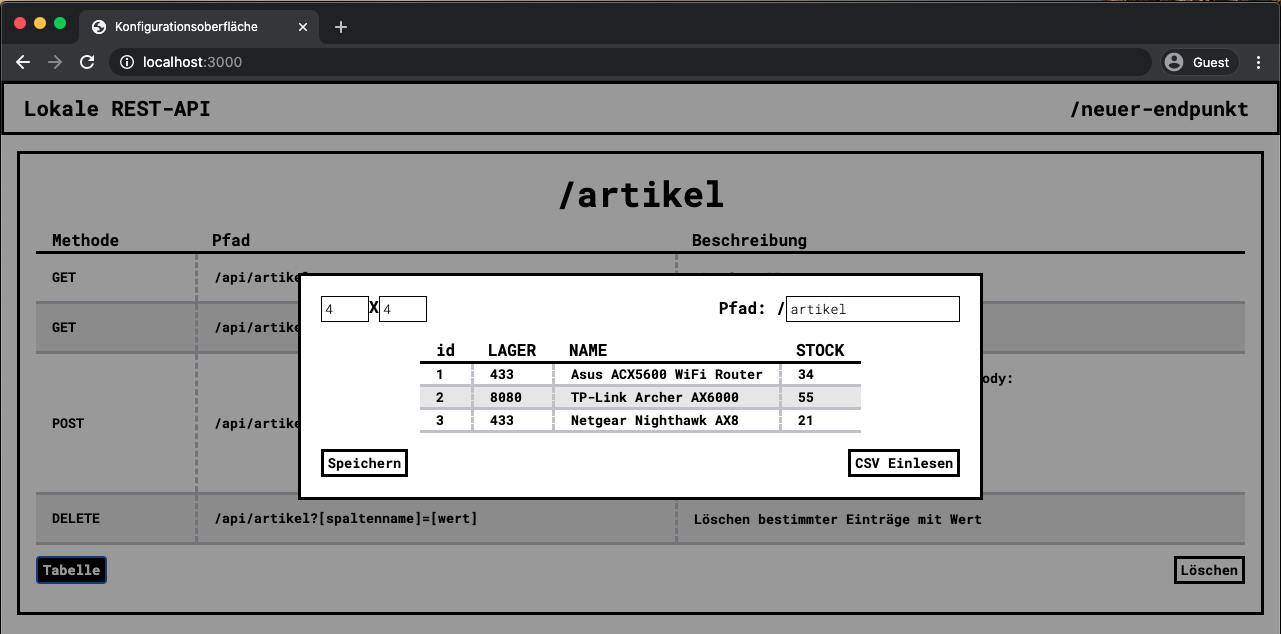
\includegraphics[width=15cm]{figures/hb_3.png}    %0.6\textwidth
    \caption{Änderung eines bestehenden Endpunktes}
    \label{fig:hb_3}
\end{figure}

Die Tabelle ist beschreibbar, was bedeutet, dass Daten durch überschreiben geändert werden können. Um gewünschte Änderungen abschließend zu persistieren, ist eine Bestätigung durch drücken des \textit{Speichern} Knopfes erforderlich.

\subsection{Erstellung eines neuen Endpunktes}

Um einen neuen Endpunkt anzulegen, wird über den Menüpunkt \textit{neuer-endpunkt} ein Modal geöffnet. Es sind mehrere Möglichkeiten zum Erstellen verfügbar. Die erste ist die manuelle Eingabe: 
Hierzu wird zunächst das Format der Datentabelle festgelegt, der Pfad des Endpunktes angegeben und anschließend Daten in die Tabelle eingetragen. Eine eindeutige ID ist nicht nötigt, da diese automatisch bei Speicherung der Tabelle erzeugt wird. Nach erfolgreicher Erstellung wird die Startübersicht inklusive der neu erstellten Tabelle angezeigt. 

\begin{figure}[H]
    \centering
    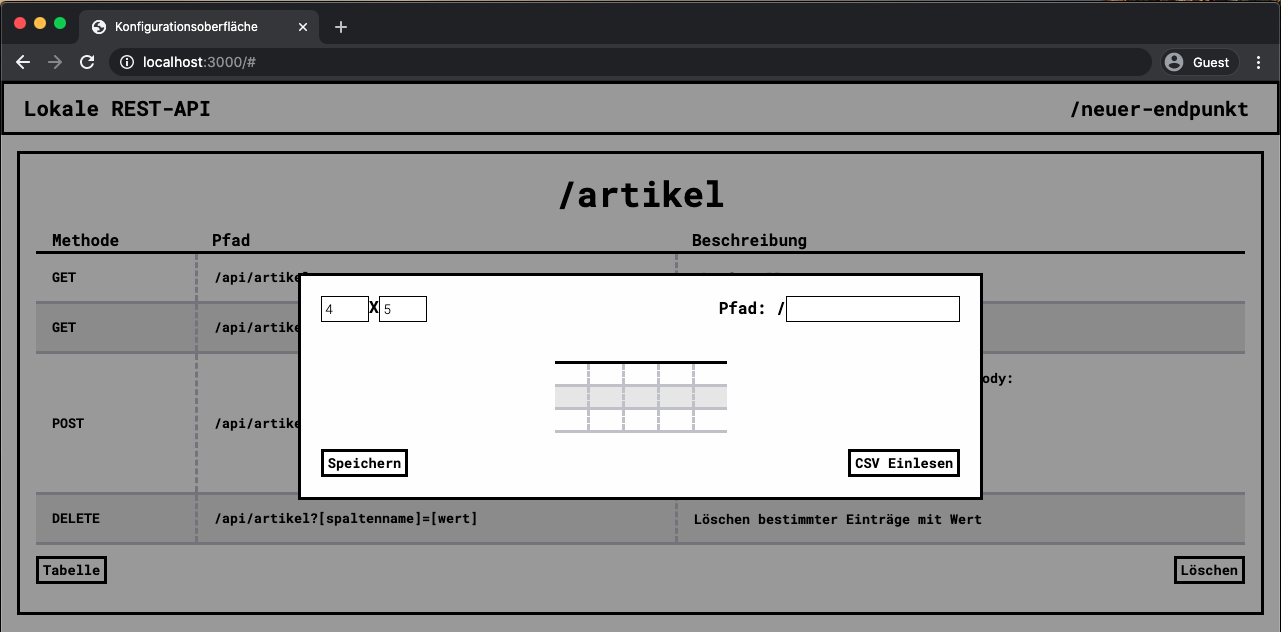
\includegraphics[width=15cm]{figures/hb_4.png}    %0.6\textwidth
    \caption{Anlegen eines neuen Endpunktes}
    \label{fig:hb_4}
\end{figure}
Weiterhin ist es möglich eine \gls{csv}-Datei einzulesen. Das einzuhaltende Format ist in \autoref{fig:hb_5} abgebildet. Die erste Zeile ist immer die Kopfzeile der Tabelle. Spalten werden durch Kommata voneinander abgegrenzt und eine neue Zeile wird durch einen Zeilenumbruch gekennzeichnet. 

\begin{figure}[H]
    \centering
    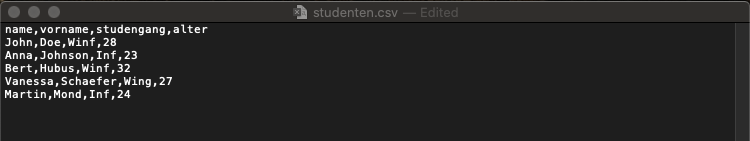
\includegraphics[width=15cm]{figures/hb_5.png}    %0.6\textwidth
    \caption{Format einer CSV-Datei}
    \label{fig:hb_5}
\end{figure}

Durch das Bestätigen der Schaltfläche \textit{CSV Einlesen} erscheint ein Dateidialog, wie in \autoref{fig:hb_6} zu sehen. Durch die Auswahl der entsprechenden Datei, wird diese eingelesen. 
\begin{figure}[H]
    \centering
    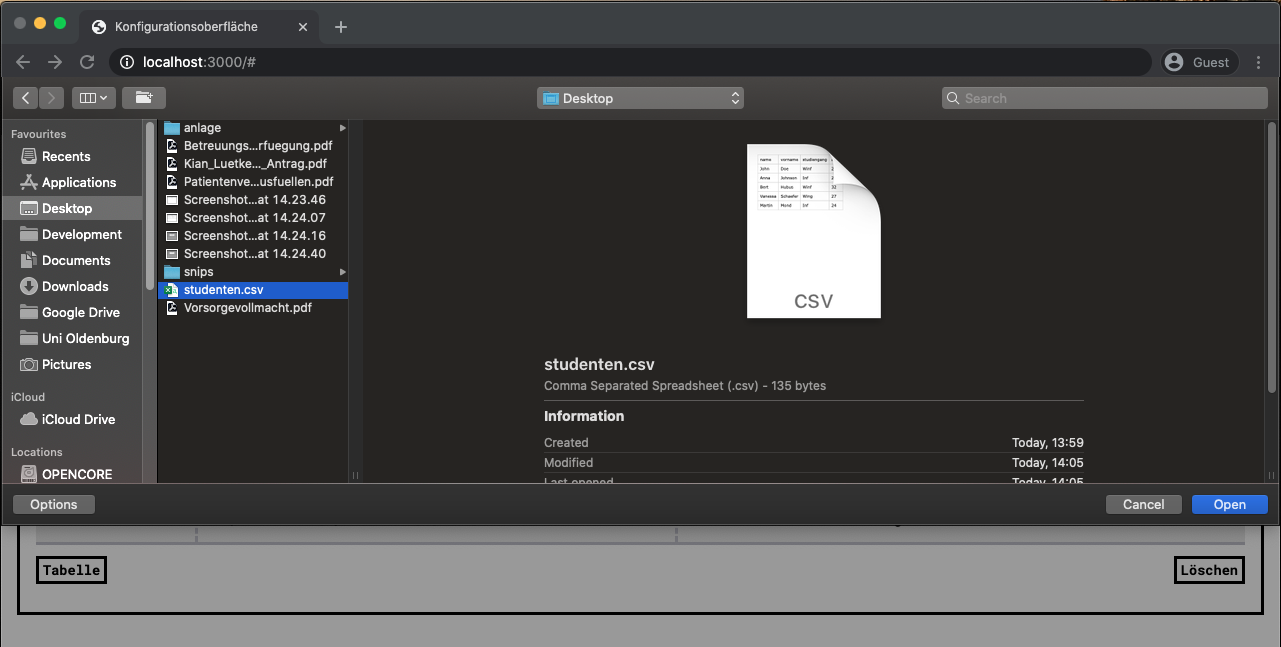
\includegraphics[width=15cm]{figures/hb_6.png}    %0.6\textwidth
    \caption{Einlesen einer CSV-Datei}
    \label{fig:hb_6}
\end{figure}

Nach erfolgreichem Hochladen der \gls{csv}-Datei erscheinen die Daten in einem neuen Modal. Hier besteht die Möglichkeit Änderungen vorzunehmen. Zudem muss der gewünschte Pfad (Name des Endpunktes) angegeben werden.

\begin{figure}[H]
    \centering
    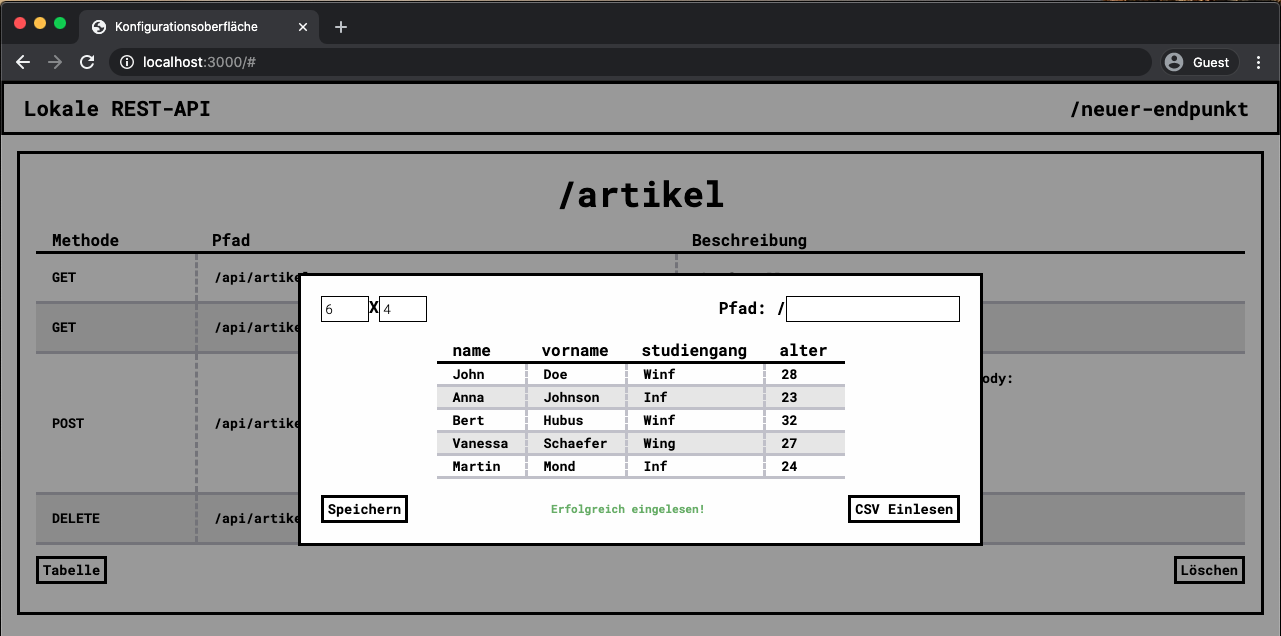
\includegraphics[width=15cm]{figures/hb_7.png}    %0.6\textwidth
    \caption{Anzeige der importierten Tabelle}
    \label{fig:hb_7}
\end{figure}

\newpage
\section{REST-API}

\subsection{Datenabfrage}

Um die erstellten Endpunkte abzufragen, müssen \gls{http}-Requests auf die entsprechende \gls{url} ausgeführt werden. Die einfachste Form ist das Konsolen Programm \textit{curl}. Dieses gehört bei den meisten Betriebssystemen zum Standard und ist auch unter dem hier verwendeten MacOS Teil des Systems \cite{DanielStenbergandContributers.2020}.

\begin{verbatim}
> curl localhost:3000/api/artikel | json_pp
{
   "message" : "Request successful",
   "status" : 200,
   "data" : [
      {
         "STOCK" : "34",
         "NAME" : "Asus ACX5600 WiFi Router",
         "LAGER" : "433",
         "id" : 1
      },
      {
         "LAGER" : "8080",
         "NAME" : "TP-Link Archer AX6000",
         "STOCK" : "55",
         "id" : 2
      },
      [...]
   ]
}
\end{verbatim}

Der obige Ausschnitt zeigt, wie ein einfacher GET-Request auf den Endpunkt \textit{artikel} ausgeführt wird.
Durch die Übergabe an das ebenfalls standardmäßig vorhandene Konsolenprogramm \textit{json\_pp} wird die Ausgabe ansprechender formatiert. Dies ist nicht zwingend notwendig, verbessert jedoch die Übersichtlichkeit. Die Ausgabe zeigt eine Nachricht, dass die Anfrage Fehlerfrei war, sowie den Status-Code 200. Zudem wird das Array \textit{data} zurückgegeben, welches die angeforderten Daten enthält.

Um nun nur einen bestimmten Artikel auszugeben wird ein querystring an den GET-Request angehängt:
\begin{verbatim}
> curl http://localhost:3000/api/artikel\?id\=1 |json_pp                                                                                                                                       
{
   "status" : 200,
   "message" : "Request successful",
   "data" : [
      {
         "LAGER" : "433",
         "NAME" : "Asus ACX5600 WiFi Router",
         "id" : 1,
         "STOCK" : "34"
      }
   ]
}
\end{verbatim}

Hervorzuheben ist, dass bei der Benutzung von \textit{curl} Ssonderzeichen, wie zum Beispiel das ? oder das \& Zeichen ein vorgestelltes / Zeichen benötigen, damit die Abfrage korrekt funktioniert. 

\subsection{Datenmanipulation: Erstellen und Löschen}
Um einen neuen Eintrag der Tabelle hinzuzufügen bedarf es eines POST-Requests. Dies beherrscht das Werkzeug \textit{curl} ebenfalls. Folgendes Listing illustriert ein solches Vorgehen:

\begin{verbatim}
> curl -d '{"LAGER": "433", "NAME": "Huawei AX3 Standard", "STOCK": "4"}' \
-H "Content-Type: application/json" \
-X POST http://localhost:3000/api/artikel | json_pp 
{
   "message" : "Ressource successfully created",
   "status" : 201,
   "data" : [
         [...]
         {
            "STOCK" : "4",
            "id" : 5,
            "LAGER" : "433",
            "NAME" : "Huawei AX3 Standard"
         }
      ]
}
\end{verbatim}

Dabei werden einige Parameter genutzt:
\begin{itemize}
    \item \textit{-d}: das d steht für data, hier wird der \gls{json}-Body übergeben. 
    \item \textit{-H}: An dieser stelle können \gls{http}-Header übergeben werden.
    \item \textit{-X}: Dieser Buchstabe steht für den Request-Typ; in diesem Fall POST.
\end{itemize}

Wie in diesem Beispiel zu sehen Antwortet die \gls{api} nicht nur mit einer Erfolgsmeldung, sondern gibt auch alle Daten zurück inklusive der neu hinzugefügten.

Schließlich fehlt noch das Löschen vorhandener Einträge. Dafür wird der \gls{http}-Request DELETE genutzt, wie folgendes Listing veranschaulicht:
\newpage
\begin{verbatim}
> curl -X DELETE http://localhost:3000/api/artikel\?id\=2 | json_pp
{
   "status" : 200,
   "data" : [
      {
         "STOCK" : "21",
         "id" : 3,
         "LAGER" : "433",
         "NAME" : "Netgear Nighthawk AX8"
      },
      {
         "NAME" : "Huawei AX3 PRO",
         "STOCK" : "12",
         "LAGER" : "433",
         "id" : 4
      },
      {
         "NAME" : "Huawei AX3 Standard",
         "LAGER" : "433",
         "id" : 5,
         "STOCK" : "4"
      }
   ],
   "message" : "Request successful"
}
\end{verbatim}

Hier lässt sich erkennen, dass wieder der -X Parameter genutzt wurde, um die Methode DELETE auszuwählen. Die \gls{api} gibt eine Erfolgsmeldung zurück  sowie die verbleibenden Daten der Tabelle.